\newpage
\section{Model analityczny}

Celem stworzonego w niniejszym rozdziale modelu analitycznego jest
zdefiniowanie, jak wyglądać będzie architektura tworzonego systemu, jakie
problemy mogą być związane z poszczególnymi elementami całości i jakie kroki
można przedsięwziąć w celu zapobieżenia najczęściej występującym i najbardziej
prawdopodobnym zagrożeniom. Aby to osiągnąć, zaprezentowano różnego rodzaju
diagramy UML, które służą jako wizualna reprezentacja architektury systemu i
pozwalają na łatwiejszą analizę stanu projektu.


\subsection{Diagram klas}



Przedstawiony na poniższym obrazku diagram klas reprezentuje wszystkie
wykorzystywane przez Zleceniodawcę elementy składające się na cały system.
Diagram ten ma znaczenie przede wszystkim dla deweloperów i osób zajmujących się
wytwarzaniem oprogramowania, tym niemniej powinien zostać zatwierdzony przed
przedstawicieli Zleceniodawcy - diagram klas jest bowiem punktem łączącym z
jednej strony wyobrażenie klienta o podziale funkcjonalności a z drugiej decyzje
projektowe podjęte przez zespół zajmujący się implementacją.

Diagram klas powinien obrazować zależności (agregacje, kompozycje, relację
dziedziczenia) pomiędzy poszczególnymi klasami na tyle szczegółowo, by osoby 
nieposiadające wykształcenia informatycznego i nieznające metod programowania
obiektowego mogłby zrozumieć zasadę podziału bez szczegółowych wyjaśnień. Z
tego też powodu na poniższym rysunku skoncentrowano się na powiązaniach pomiędzy
poszczególnymi klasami a nie na nazywaniu i przedstawianiu atrybutów i metod
poszczególnych klas. Nie stanowią one żadnej wartości z punktu widzenia
Zleceniodawcy a mogą stanowić ograniczenie i usztywnienie schematu dla
deweloperów, którzy lepiej znają metody dostarczania funkcjonalności i będą
mogli lepiej modyfikować schemat w zależności od potrzeb, nie naruszając
jednocześnie warunków umowy. Wszystkie atrybuty czy operacje ważne z punktu
widzenia Zleceniodawcy, które mogą mieć wpływ na ocenę projektu zostały
umieszczone na diagramie.

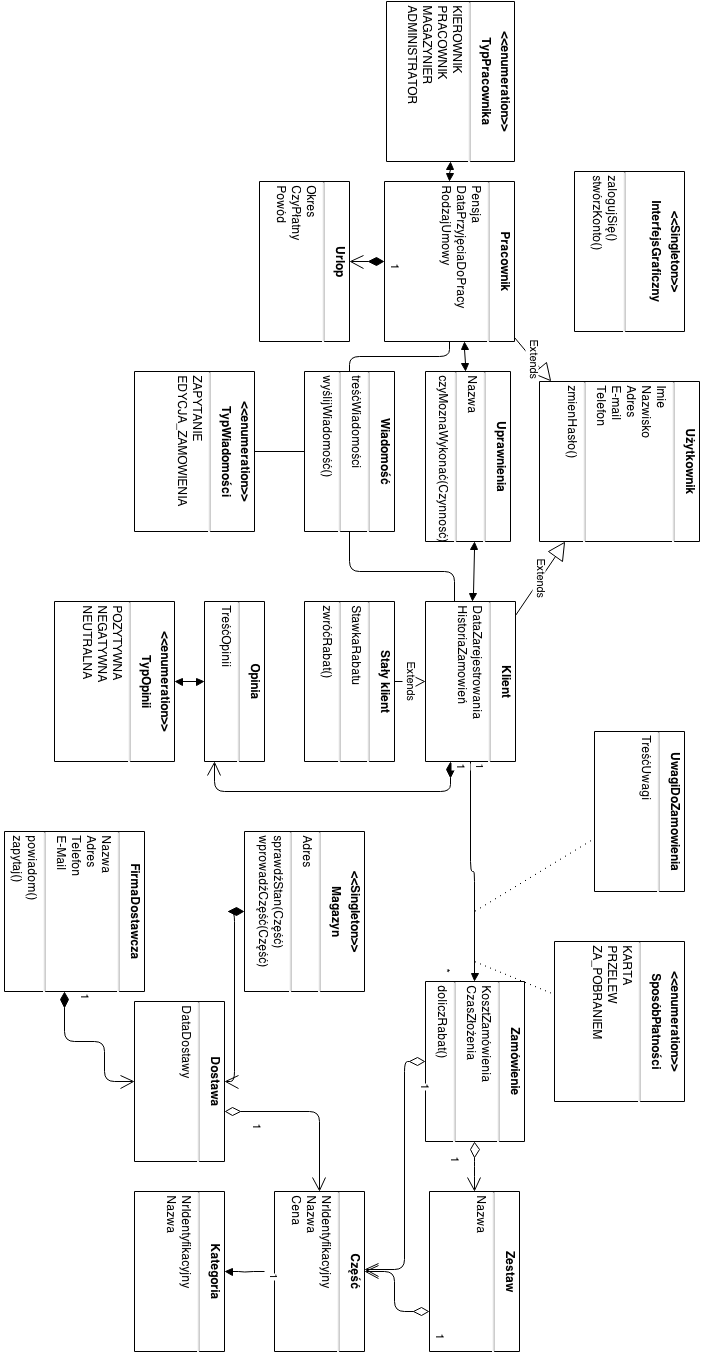
\includegraphics[width=\textwidth,
height=0.8\textheight]{graphics/ClassDiagram.png}


\newpage
Opis klas na przedstawionym diagramie:

\begin{description}
	\item[Użytkownik] \hfill \\
		Klasa abstrakcyjna, będąca bazową dla klas Klient i Pracownik, przechowuje
		informacje dotyczące danej osoby - imię, nazwisko, adres e-mail itp.
	\item[Pracownik] \hfill \\
	 	Osoba z obsługi sklepu, odpowiedzialna za realizację i zarządzanie
	 	zamówieniami
	\item[Stały klient] \hfill \\
		Osoba charakteryzująca się dużą liczbą zamówień bądź długim czasem obecności
		na stronie (czas liczony od czasu rejestracji)
	\item[Klient] \hfill \\
		Osoba składająca zamówienia w sklepie, edytująca swoje zamówienia i opłacająca
		je
	\item[Typ pracownika] \hfill \\
		Enumeracja, będąca oznaczeniem rodzaju pracownika (Szeregowy Pracownik,
		Kierownik itp.)
	\item[Urlop] \hfill \\
		Obsługa urlopów dla pracowników pod kątem czasu ich trwania, momentu ich
		rozpoczęcia (i zakończenia) itp.
	\item[Uprawnienia] \hfill \\
		Obsługa uprawnień zarówno dla pracowników jak i klientów. Pozwala na
		ustalanie, kto ma jakie uprawnienia do edycji i podglądu danych
	\item[Wiadomość] \hfill \\
		Treści przesyłane pomiędzy pracownikami i klientami, służące do przekazywania
		informacji na temat zamówień
	\item[Typ wiadomości] \hfill \\
		Enumeracja, jaki rodzaj wiadomości jest przekazywany (Zapytanie, Edycja
		Zamówienia itp.)
	\item[Opinia] \hfill \\
		Tekst na temat zamówienia, ocena poprawności i jakości realizacji zamówienia
	\item[Typ opinii] \hfill \\
		Enumeracja, jaka opinia została wydana (Pozytywna, Negatywna, Neutralna)
	\item[Zamówienie] \hfill \\
		Informacje na temat złożonego przez klienta Zamówienia
	\item[Uwagi do zamówienia] \hfill \\
		Wszelkiego rodzaju informacje, jakie klient chce zawrzeć w momencie złożenia
		zamówienia - na przykład zaznaczanie wysyłki jako prezent, ustalenie, przed
		jakim terminem zamówienie nie powinno być wysłane, czy możliwy jest odbiór
		osobisty itp.
	\item[Sposób płatności] \hfill \\
		Informacja, jak użytkownik chce zapłacić za złożone zamówienie - inaczej
		wygląda procesowanie zapłaty kartą (wysłanie następuje dopiero po wpłynięciu
		pieniędzy, opłata za pobraniem jest uiszczana dopiero po wysłaniu)
	\item[Część] \hfill \\
		Pojedyncza część rowerowa wraz z informacjami na jej temat - rozmiar, nazwa,
		cena itp.
	\item[Zestaw] \hfill \\
		Złożenie kilku części w jeden, funkcjonalnie sprawny rower. Przechowuje
		informację o tym, jakie części są wymagane, ile ma ich być (rama - 1, pedały
		-2, przerzutki - nieokreślone)
	\item[Kategoria] \hfill \\
		Informacja, do jakiej kategorii zaliczana jest dana część. Jest to pomocne do
		układania zestawów i sprawdzania ich poprawności
	\item[Dostawa] \hfill \\
		Informacje na temat jednej dostawy, jakie części i w jakiej ilości zostały
		dostarczone i kiedy
	\item[Firma dostawcza] \hfill \\
		Informacje na temat firmy, która dostarcza części - dane kontaktowe, adres
		oraz jakie części są w stanie dostarczyć
	\item[Magazyn] \hfill \\
		Klasa pozwalająca na zarządzanie częściami przechowywanymi w magazynie,
		sprawdzanie ich dostępności oraz aktualizacja stanu
	\item[Interfejs graficzny] \hfill \\
		Klasa będąca ``wejściem'' do diagramu klas, odpowiedzialna za podstawową,
		wstępną integrację z użytkownikiem
\end{description}
\subsection{Model bazy danych}

Ważnym elementem tworzonego systemu informatycznego jest baza danych
przechowująca wszystkie informacje, które powinny być pamiętane trwale. Jak
opisano w części dotyczącej sprzętu, wszystkie informacje powinny być
przechowywane redundantnie, na przynajmniej dwóch niezależnych od siebie
macierzach dyskowych. Pozwoli to na minimalizację problemów związanych z
ewentualnym awariami i chwilowymi przerwami w dostępności.

W czasie tworzenia projektu bazy danych opierano się przede wszystkim na
stworzonym wcześniej diagramie klas. Większość klas została zamieniona na
odpowiadające im tabele w bazie danych. W przypadku związków wiele-do-wielu
konieczne było stworzenie dodatkowych tabel ``rozbijających''. Enumeracje
zostały zamienione na osobne tabele tylko w przypadkach, w których
istniało prawdopodobieństwo, że w następnych latach będą rozbudowane o kolejne
pozycje. W przypadku enumeracji stałych zostały one rozwiązane jako ograniczenia
(ang. constraints) na odpowiednich tabelach.

Poniżej zaprezentowano model bazy danych wykorzystywanej w tworzonym systemie:

\clearpage
\begin{figure}[h!]
  \centering
    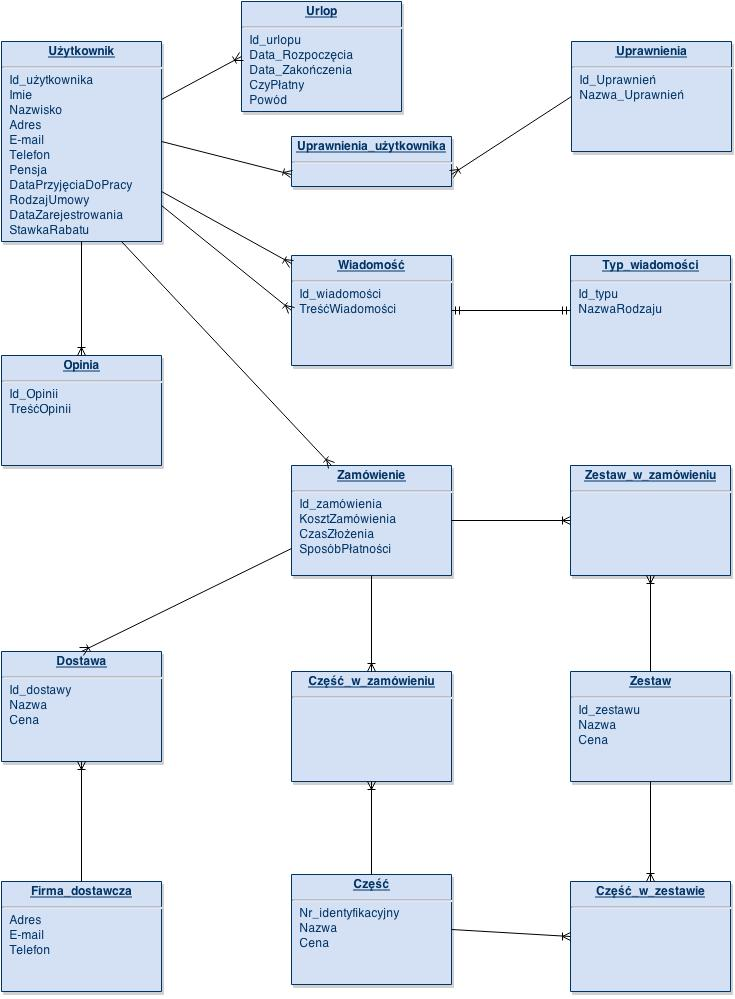
\includegraphics[width=\textwidth,
    height=0.9\textheight]{graphics/Entity_Diagram.jpg}
  \caption{Diagram encji w tworzonym modelu bazodanowym}
\end{figure}


Logiczny model bazy danych składa się z następujących tabel:

\begin{enumerate}
  \item Użytkownik
  	\begin{enumerate}
  	  \item Odpowiada za przechowywanie informacji o wszystkich osobach
  	  zapisanych w systemie, zarówno pracownikach sklepu jak i użytkownikach.
  	  Rozwiązuje problem przeniesienia dziedziczenia z modelu obiektowego do
  	  modelu bazodanowego.
  	  \item Decyzja o przechowywaniu danych o klientach i pracownikach w jednej
  	  tabeli podyktowana jest chęcią przyśpieszenia wyszukiwania osób.
  	\end{enumerate}
  	{\footnotesize
  	\begin{longtable}{|p{3cm}|p{5cm}|p{2.5cm}|p{2.5cm}|}
  	\hline
  	\textbf{Nazwa atrybutu} & \textbf{Znaczenie atrybutu} & \textbf{Typ danych} &
  	\textbf{Ograniczenia} \\
  	\hline
  	Id\_użytkownika & PRIMARY KEY & Integer(7,0) & NOT NULL, UNIQUE \\
	\hline
  	Imię & Pierwsze imię użytkownika & VARCHAR2(30) & - \\
	\hline
  	Nazwisko & Nazwisko użytkownika & VARCHAR2(50) & - \\
	\hline
  	Adres & Dane dotyczące wysyłki & VARCHAR2(80) & - \\
	\hline
  	E-mail & Adres internetowy do korespondencji & VARCHAR2(30) & REGEXP LIKE
  	\texttt{(\b[A-Z0-9.\_\%+-]}
  	\newline
  	\texttt{+@[A-Z0-9.-]+}
  	\newline
  	\texttt{\.[A-Z]\{2,4\}\b)}
  	 \\
 	\hline
  	Telefon & Telefon kontaktowy do korespondencji & Integer(9,0) & - \\
 	\hline
  	Pensja & Wynagrodzenie pracownika & Integer(10,2) & - \\
	\hline
  	Data przyjęcia do pracy & Data podpisania umowy & Date & - \\
	\hline
  	Rodzaj umowy & Na jakiej umowie jest zatrudniony pracownik & VARCHAR2(15) &
  	CHECK IN (O PRACE, O DZIEŁO, ZLECENIE) \\
	\hline
  	Data\_zarejestrowania & Kiedy klient zarejestrował się w systemie &
  	Date & -
  	\\
	\hline
  	Stawka\_rabatu & Dostępna dla stałych klientów & Integer(2,0) & CHECK <100 \&
  	>0
  	\\
    \hline
	\caption{Opis atrybutów w tabeli Użytkownik}
	\end{longtable}}
 \item Uprawnienia
  	\begin{enumerate}
  	  \item Tabela zawierająca uprawnienia, jakie można nadać użytkownikom,
  	  zarówno klientom jak i pracownikom
  	  \item Zbiory uprawnień są różne dla klientów i pracowników, jednak mogą
  	  zawierać części wspólne (np. prawo do przeglądania produktów)
  	\end{enumerate}
  	{\footnotesize
  	\begin{longtable}{|p{3cm}|p{5cm}|p{2.5cm}|p{2.5cm}|}
  	\hline
  	\textbf{Nazwa atrybutu} & \textbf{Znaczenie atrybutu} & \textbf{Typ danych} &
  	\textbf{Ograniczenia} \\
  	\hline
  	Id\_uprawnień & PRIMARY KEY & Integer(2,0) & NOT NULL, UNIQUE \\
  	\hline
  	Nazwa\_uprawnień & Nazwa dodana dla wygody użytkowników & VARCHAR2(30) & - 
  	\\
  	\hline
	\caption{Opis atrybutów w tabeli Uprawnienia}
	\end{longtable}}
  \item Uprawnienia\_użytkownika
  	\begin{enumerate}
  	  \item Tabela rozbijająca związek wiele-do-wielu pomiędzy tabelami
  	  Uprawnienia i Użytkownik
  	  \item Nie zawiera innych atrybutów niż klucze obce
  	\end{enumerate}
  	{\footnotesize
  	\begin{longtable}{|p{3cm}|p{5cm}|p{2.5cm}|p{2.5cm}|}
  	\hline
  	\textbf{Nazwa atrybutu} & \textbf{Znaczenie atrybutu} & \textbf{Typ danych} &
  	\textbf{Ograniczenia} \\
  	\hline
  	ID\_użytkownika & FOREIGN KEY REFERENCES Użytkownik.ID\_użytkownika  &
  	Integer (7,0) & NOT NULL
  	\\
  	\hline
  	ID\_uprawnień & FOREIGN KEY REFERENCES Uprawnienia.ID\_uprawnień &
  	Integer(2,0)) & NOT NULL
  	\\
  	\hline
	\caption{Opis atrybutów w tabeli Uprawnienia\_użytkownika}
	\end{longtable}}
  \item Urlop
  	\begin{enumerate}
  	  \item Tabela pozwalająca na przechowanie danych o urlopach pracowniczych
  	  \item Zawiera informacje na temat czasu trwania, daty rozpoczęcia i
  	  zakończenia oraz inne dane
  	\end{enumerate}
  	{\footnotesize
  	\begin{longtable}{|p{3cm}|p{5cm}|p{2.5cm}|p{2.5cm}|}
  	\hline
  	\textbf{Nazwa atrybutu} & \textbf{Znaczenie atrybutu} & \textbf{Typ danych} &
  	\textbf{Ograniczenia} \\
  	\hline
  	ID\_pracownika & FOREIGN KEY REFERENCES Użytkownik.ID\_użytkownika  &
  	Integer(7,0) & NOT NULL
  	\\
  	\hline
  	ID\_urlopu & PRIMARY KEY & Integer(5,0) & NOT NULL, UNIQUE  \\
  	\hline
  	Data\_rozpoczęcia & Data rozpoczęcia urlopu & Date & -  \\
  	\hline
  	Data\_zakończenia & Data zakończenia urlopu & Date & Data\_zakończenia >=
  	Data\_rozpoczęcia
  	\\
  	\hline
  	CzyPłatny & Informacja czy urlop jest płatny czy nie & Integer(1,0) & CHECK
  	IN (1,0) \\
  	\hline
  	Powód & Jaki jest powód urlopu (wypoczynkowy, leczniczy itp.) & VARCHAR2(100)
  	& - \\
  	\hline
	\caption{Opis atrybutów w tabeli Urlop}
	\end{longtable}}
  \item Wiadomość
  	\begin{enumerate}
  	  \item Wiadomość przekazywana pomiędzy pracownikami i klientami lub pomiędzy
  	  pracownikami
  	  \item Służy do usprawnienia wymiany informacji
  	\end{enumerate}
  	{\footnotesize
  	\begin{longtable}{|p{3cm}|p{5cm}|p{2.5cm}|p{2.5cm}|}
  	\hline
  	\textbf{Nazwa atrybutu} & \textbf{Znaczenie atrybutu} & \textbf{Typ danych} &
  	\textbf{Ograniczenia} \\
  	\hline
  	Id\_użytkownika1 & FOREIGN KEY REFERENCES Użytkownik.Id\_użytkownika  &
  	Integer(7,0) & NOT NULL
  	\\
  	\hline
  	Id\_użytkownika2 & FOREIGN KEY REFERENCES Użytkownik.Id\_użytkownika &
  	Integer(7,0) & NOT NULL
  	\\
  	\hline
  	Id\_wiadomości & PRIMARY KEY & Integer(9,0) & NOT NULL, UNIQUE  \\
  	\hline
  	Treść\_wiadomości & Wiadomość przekazywana między użytkownikami &
  	VARCHAR2(500) & -
  	\\
  	\hline
	\caption{Opis atrybutów w tabeli Wiadomość}
	\end{longtable}}
  \item Typ\_Wiadomości
  	\begin{enumerate}
  	  \item Reprezentacja enumeracji TYP\_WIADOMOŚCI z modelu obiektowego
  	  \item Stworzona jako osobna tabela z uwagi na możliwość rozszerzania typów 
  	\end{enumerate}
  	{\footnotesize
  	\begin{longtable}{|p{3cm}|p{5cm}|p{2.5cm}|p{2.5cm}|}
  	\hline
  	\textbf{Nazwa atrybutu} & \textbf{Znaczenie atrybutu} & \textbf{Typ danych} &
  	\textbf{Ograniczenia} \\
  	\hline
  	Id\_wiadomości & FOREIGN KEY REFERENCES Wiadomość.Id\_wiadomości  &
  	Integer(9,0) & NOT NULL
  	\\
  	\hline
  	Id\_typu & PRIMARY KEY & Integer(2,0) & NOT NULL, UNIQUE  \\
  	\hline
  	Nazwa\_rodzaju & Nazwa stworzona dla wygody użytkowników & VARCHAR2(20) &
  	-
  	\\
  	\hline
	\caption{Opis atrybutów w tabeli Typ\_wiadomości}
	\end{longtable}}
  \item Opinia
  	\begin{enumerate}
  	  \item Opinie wystawiane są przez klientów po odebraniu zamówienia
  	  \item Mogą dotyczyć zarówno zamówienia, pojedynczej części jak i ogólnie
  	  sklepu
  	  \item Z tego też powodu nie istnieje związek pomiędzy tabelą Opinia a
  	  tabelą Zamówienie czy Część
  	\end{enumerate}
  	{\footnotesize
  	\begin{longtable}{|p{3cm}|p{5cm}|p{2.5cm}|p{2.5cm}|}
  	\hline
  	\textbf{Nazwa atrybutu} & \textbf{Znaczenie atrybutu} & \textbf{Typ danych} &
  	\textbf{Ograniczenia} \\
  	\hline
  	Id\_użytkownika & FOREIGN KEY REFERENCES Użytkownik.Id\_użytkownika &
  	Integer(7,0) & NOT NULL
  	\\
  	\hline
  	Id\_Opinii & PRIMARY KEY & Integer(9,0) & NOT NULL, UNIQUE  \\
  	\hline
  	Treść\_opinii & Opinia przedstawiona przez użytkownika & VARCHAR2(500) & - \\
  	\hline
	\caption{Opis atrybutów w tabeli Opinia}
	\end{longtable}}
  \item Zamówienie
  	\begin{enumerate}
  	  \item Tabela opisująca zamówienie złożone przez klienta
  	  \item Może się składać zarówno ze zestawów (złożonych z części) jak i z
  	  samych części
  	\end{enumerate}
  	{\footnotesize
  	\begin{longtable}{|p{3cm}|p{5cm}|p{2.5cm}|p{2.5cm}|}
  	\hline
  	\textbf{Nazwa atrybutu} & \textbf{Znaczenie atrybutu} & \textbf{Typ danych} &
  	\textbf{Ograniczenia} \\
  	\hline
  	Id\_użytkownika & FOREIGN KEY REFERENCES Użytkownik.Id\_użytkownika  &
  	Integer(7,0) & -
  	\\
  	\hline
  	Id\_zamówienia & PRIMARY KEY & Integer(9,0) & NOT NULL, UNIQUE  \\
  	\hline
  	Koszt\_zamówienia & Całkowity koszt zamówienia wraz z wysyłką & Integer(7,2))
  	& -
  	\\
  	\hline
  	Czas złożenia & Kiedy zamówienie zostało złożone (ma znaczenie przy czasie
  	realizacji) & Date & -
  	\\
 	\hline
  	Sposób płatności & Jak użytkownik opłaci zamówienie (kartą, za pobraniem
  	itp.) & VARCHAR2(30) & -
  	\\
  	\hline
	\caption{Dostępne aplikacje mobilne}
	\end{longtable}}
  \item Zestaw\_w\_zamówieniu
  	\begin{enumerate}
  	  \item Tabela rozbijająca związek wiele-do-wielu pomiędzy tabelami Zestaw
  	  oraz Zamówienie
  	  \item Nie posiada własnych atrybutów poza kluczami obcymi
  	\end{enumerate}
  	{\footnotesize
  	\begin{longtable}{|p{3cm}|p{5cm}|p{2.5cm}|p{2.5cm}|}
  	\hline
  	\textbf{Nazwa atrybutu} & \textbf{Znaczenie atrybutu} & \textbf{Typ danych} &
  	\textbf{Ograniczenia} \\
  	\hline
  	Id\_zamówienia & FOREIGN KEY REFERENCES Zamówienie.Id\_zamówienia  &
  	Integer(9,0) & NOT NULL
  	\\
  	\hline
  	Id\_zestawu & FOREIGN KEY REFERENCES Zestaw.Id\_zestawu & Integer(4,0) & NOT
  	NULL
  	\\
  	\hline
	\caption{Opis atrybutów w tabeli Zestaw\_w\_zamówieniu}
	\end{longtable}}
  \item Dostawa
  	\begin{enumerate}
  	  \item Opis informacji, z jakiej dostawy możliwe jest zebranie części do
  	  konkretnego zamówienia
  	  \item Dostawy tego rodzaju określane są przez firmy dostawcze w reakcji na
  	  zapotrzebowanie ze strony sklepu (już po złożeniu zamówienia)
  	\end{enumerate}
  	{\footnotesize
  	\begin{longtable}{|p{3cm}|p{5cm}|p{2.5cm}|p{2.5cm}|}
  	\hline
  	\textbf{Nazwa atrybutu} & \textbf{Znaczenie atrybutu} & \textbf{Typ danych} &
  	\textbf{Ograniczenia} \\
  	\hline
  	Id\_firmy & FOREIGN KEY REFERENCES Firma\_dostawcza.Id\_firmy & Integer(4,0)
  	& NOT NULL \\
  	\hline
  	Id\_zamówienia & FOREIGN KEY REFERENCES
  	Zamówienie.Id\_zamówienia & Integer(9,0) & NOT NULL
  	\\
  	\hline
  	Id\_dostawy & PRIMARY KEY & Integer(8,0) & NOT NULL, UNIQUE  \\
  	\hline
  	Nazwa & Nazwa kodowa dostawy (przydatna przy identyfikacji) & VARCHAR2(50) &
  	-
  	\\
  	\hline
  	Cena & Całkowity koszt dostawy (koszt zamówienia + koszt transportu) & 
  	Integer(7,2) & -
  	\\
  	\hline
	\caption{Opis atrybutów w tabeli Dostawa}
	\end{longtable}}
  \item Firma\_dostawcza
  	\begin{enumerate}
  	  \item Opis firmy dostawczej, która dostarcza potrzebne do zamówienia
  	  produkty
  	\end{enumerate}
  	{\footnotesize
  	\begin{longtable}{|p{3cm}|p{5cm}|p{2.5cm}|p{2.5cm}|}
  	\hline
  	\textbf{Nazwa atrybutu} & \textbf{Znaczenie atrybutu} & \textbf{Typ danych} &
  	\textbf{Ograniczenia} \\
  	\hline
  	Id\_firmy & PRIMARY KEY  & Integer(4,0) & NOT NULL, UNIQUE \\
  	\hline
  	Telefon & Numer do korespondencji & VARCHAR2(11) & -  \\
  	\hline
  	Adres & Adres firmy (lub jej magazynu) & VARCHAR2(50) & -  \\
  	\hline
  	E-mail & Adres internetowy do korespondencji & VARCHAR2(30) & REGEXP LIKE
  	\texttt{(\b[A-Z0-9.\_\%+-]}
  	\newline
  	\texttt{+@[A-Z0-9.-]+}
  	\newline
  	\texttt{\.[A-Z]\{2,4\}\b)}
  	\\
  	\hline
	\caption{Opis atrybutów w tabeli Firma\_dostawcza}
	\end{longtable}}
  \item Część
  	\begin{enumerate}
  	  \item Pojedyncza część rowerowa (pedał, siodełko, przerzutka itp.)
  	  \item Z pojedynczych części składają się zarówno zestawy jak i zamówienia
  	\end{enumerate}
  	{\footnotesize
  	\begin{longtable}{|p{3cm}|p{5cm}|p{2.5cm}|p{2.5cm}|}
  	\hline
  	\textbf{Nazwa atrybutu} & \textbf{Znaczenie atrybutu} & \textbf{Typ danych} &
  	\textbf{Ograniczenia} \\
  	\hline
  	Nr\_identyfikacyjny & PRIMARY KEY & Integer(6,0) & NOT NULL, UNIQUE \\
  	\hline
  	Nazwa & Przydatna przy wyszukiwaniu & VARCHAR2(60) & \\
  	\hline
  	Cena  & Koszt części w danym momencie czasowym & Integer(7,2) &  \\
  	\hline
	\caption{Opis atrybutów w tabeli Część}
	\end{longtable}}
  \item Zestaw
  	\begin{enumerate}
  	  \item Zestawy składają się z dwóch lub więcej części
  	  \item Ich cena może być niższa niż sumaryczny koszt części (na przykład
  	  wskutek promocji)
  	\end{enumerate}
  	{\footnotesize
  	\begin{longtable}{|p{3cm}|p{5cm}|p{2.5cm}|p{2.5cm}|}
  	\hline
  	\textbf{Nazwa atrybutu} & \textbf{Znaczenie atrybutu} & \textbf{Typ danych} &
  	\textbf{Ograniczenia} \\
  	\hline
  	Id\_zestawu & PRIMARY KEY  & Integer(5,0) & NOT NULL, UNIQUE \\
  	\hline
  	Nazwa & Nazwa zestawu, przydatna przy przeglądaniu & VARCHAR2(60) & -  \\
  	\hline
	\caption{Opis atrybutów w tabeli Zestaw}
	\end{longtable}}
  \item Część\_w\_zamówieniu
  	\begin{enumerate}
  	  \item Tabela pomocnicza, rozbijająca związek wiele-do-wielu pomiędzy
  	  tabelami Część i Zamówienie
  	  \item Nie zawiera własnych atrybutów poza kluczami obcymi
  	\end{enumerate}
  	{\footnotesize
  	\begin{longtable}{|p{3cm}|p{5cm}|p{2.5cm}|p{2.5cm}|}
  	\hline
  	\textbf{Nazwa atrybutu} & \textbf{Znaczenie atrybutu} & \textbf{Typ danych} &
  	\textbf{Ograniczenia} \\
  	\hline
  	Nr\_identyfikacyjny & FOREIGN KEY REFERENCES Część.Nr\_identyfikacyjny  &
  	Integer(6,0) & NOT NULL
  	\\
  	\hline
  	Id\_zamówienia & FOREIGN KEY REFERENCES Zamówienie.Id\_zamówienia &
  	Integer(9,0) & NOT NULL
  	\\
  	\hline
	\caption{Opis atrybutów w tabeli Część\_w\_zamówieniu}
	\end{longtable}}
  \item Część\_w\_zestawie
  	\begin{enumerate}
  	  \item Tabela rozbijająca związek wiele-do-wielu pomiędzy tabelami Część i
  	  Zestaw
  	  \item Nie posiada własnych atrybutów poza kluczami obcymi
  	\end{enumerate}
  	{\footnotesize
  	\begin{longtable}{|p{3cm}|p{5cm}|p{2.5cm}|p{2.5cm}|}
  	\hline
  	\textbf{Nazwa atrybutu} & \textbf{Znaczenie atrybutu} & \textbf{Typ danych} &
  	\textbf{Ograniczenia} \\
  	\hline
  	Nr\_identyfikacyjny & FOREIGN KEY REFERENCES Część.Nr\_identyfikacyjny  &
  	Integer(6,0) & NOT NULL
  	\\
  	\hline
  	Id\_zestawu & FOREIGN KEY REFERENCES Zestaw.Id\_zestawu & Integer(5,0) &
  	NOT NULL
  	\\
  	\hline
	\caption{Opis atrybutów w tabeli Część\_w\_zestawie}
	\end{longtable}}
\end{enumerate}
